% Options for packages loaded elsewhere
\PassOptionsToPackage{unicode}{hyperref}
\PassOptionsToPackage{hyphens}{url}
\documentclass[
  11pt,
  a4paper,
]{article}
\usepackage{xcolor}
\usepackage[margin=25mm]{geometry}
\usepackage{amsmath,amssymb}
\setcounter{secnumdepth}{-\maxdimen} % remove section numbering
\usepackage{iftex}
\ifPDFTeX
  \usepackage[T1]{fontenc}
  \usepackage[utf8]{inputenc}
  \usepackage{textcomp} % provide euro and other symbols
\else % if luatex or xetex
  \usepackage{unicode-math} % this also loads fontspec
  \defaultfontfeatures{Scale=MatchLowercase}
  \defaultfontfeatures[\rmfamily]{Ligatures=TeX,Scale=1}
\fi
\usepackage{lmodern}
\ifPDFTeX\else
  % xetex/luatex font selection
\fi
% Use upquote if available, for straight quotes in verbatim environments
\IfFileExists{upquote.sty}{\usepackage{upquote}}{}
\IfFileExists{microtype.sty}{% use microtype if available
  \usepackage[]{microtype}
  \UseMicrotypeSet[protrusion]{basicmath} % disable protrusion for tt fonts
}{}
\makeatletter
\@ifundefined{KOMAClassName}{% if non-KOMA class
  \IfFileExists{parskip.sty}{%
    \usepackage{parskip}
  }{% else
    \setlength{\parindent}{0pt}
    \setlength{\parskip}{6pt plus 2pt minus 1pt}}
}{% if KOMA class
  \KOMAoptions{parskip=half}}
\makeatother
\usepackage{longtable,booktabs,array}
\usepackage{caption}

\newcounter{none} % for unnumbered tables
\usepackage{calc} % for calculating minipage widths
% Correct order of tables after \paragraph or \subparagraph
\usepackage{etoolbox}
\makeatletter
\patchcmd\longtable{\par}{\if@noskipsec\mbox{}\fi\par}{}{}
\makeatother
% Allow footnotes in longtable head/foot
\IfFileExists{footnotehyper.sty}{\usepackage{footnotehyper}}{\usepackage{footnote}}
\makesavenoteenv{longtable}
\usepackage{graphicx}
\makeatletter
\newsavebox\pandoc@box
\newcommand*\pandocbounded[1]{% scales image to fit in text height/width
  \sbox\pandoc@box{#1}%
  \Gscale@div\@tempa{\textheight}{\dimexpr\ht\pandoc@box+\dp\pandoc@box\relax}%
  \Gscale@div\@tempb{\linewidth}{\wd\pandoc@box}%
  \ifdim\@tempb\p@<\@tempa\p@\let\@tempa\@tempb\fi% select the smaller of both
  \ifdim\@tempa\p@<\p@\scalebox{\@tempa}{\usebox\pandoc@box}%
  \else\usebox{\pandoc@box}%
  \fi%
}
% Set default figure placement to htbp
\def\fps@figure{htbp}
\makeatother
\setlength{\emergencystretch}{3em} % prevent overfull lines
\providecommand{\tightlist}{%
  \setlength{\itemsep}{0pt}\setlength{\parskip}{0pt}}
\usepackage[T1]{fontenc}
\DeclareUnicodeCharacter{2212}{\ensuremath{-}}
\DeclareUnicodeCharacter{2260}{\ensuremath{\ne}}
\DeclareUnicodeCharacter{2248}{\ensuremath{\approx}}
\DeclareUnicodeCharacter{2264}{\ensuremath{\le}}
\DeclareUnicodeCharacter{2265}{\ensuremath{\ge}}
\usepackage{lmodern}
\usepackage{microtype}
\usepackage{placeins}
\usepackage{longtable,booktabs,array}
\usepackage{etoolbox}
\pretocmd{\section}{\FloatBarrier}{}{}
\AtBeginEnvironment{longtable}{\small\setlength{\tabcolsep}{3pt}}
\AtBeginDocument{\hypersetup{unicode=true,pdfsubject={Preliminary manuscript; not peer reviewed}}}
\usepackage{bookmark}
\IfFileExists{xurl.sty}{\usepackage{xurl}}{} % add URL line breaks if available
\urlstyle{same}
% fallback for those not using the hyperref driver hyperxmp:
\makeatletter
\@ifundefined{xmpquote}{\newcommand{\xmpquote}[1]{#1}}{}
\makeatother
\hypersetup{
  pdftitle={Reversible JPEG Coefficient Swapping: Reducing Restoration-Information Cost with ARPT and Confidence-Guided Carrier Selection},
  pdfauthor={Shao-An Chien},
  hidelinks,
  pdfcreator={LaTeX via pandoc}}

\title{Reversible JPEG Coefficient Swapping: Reducing
Restoration-Information Cost with ARPT and Confidence-Guided Carrier
Selection}
\author{Shao-An Chien}
\date{Preliminary manuscript --- not peer reviewed}

\begin{document}
\maketitle

Date: 2026-10-05

Department of Computer Science and Information Engineering, Ming Chuan
University\\
Email: \texttt{11360483@me.mcu.edu.tw}, \texttt{rex99075@gmail.com}

\section*{Abstract}\label{abstract}
\addcontentsline{toc}{section}{Abstract}

Reversible watermarking attaches authorization information to an image
for copyright protection and restores the original image after
extraction for subsequent use. JPEG is a common format for image
sharing. Existing AC-pair swapping methods can provide high watermark
robustness, but restoring the original image requires recording
prediction errors; reducing these errors therefore lowers the
restoration-information cost.

This paper proposes an Antisymmetric Residual-Pairing Transformer (ARPT)
that compares two candidate coefficient-pair arrangements to predict the
swap state. Carriers are selected according to prediction confidence to
reduce the number of errors that must be recorded. The remaining errors
are stored as a lossless correction map in the marked JPEG, allowing the
receiver to restore the original image.

Experiments show that ARPT achieves approximately 94.7\% swap-state
classification accuracy. Confidence-guided carrier selection reduces the
error rate among selected carriers from 5.45\% to 0.66\%, lowers the
restoration-information cost, and permits exact restoration of the
original quantized coefficients and decoded pixels.

\textbf{Keywords:} reversible watermarking; JPEG; ARPT;
confidence-guided carrier selection; correction map; overhead-adjusted
payload

\section*{1. Introduction}\label{introduction}
\addcontentsline{toc}{section}{1. Introduction}

Digital watermarking embeds copyright labels or authorization
information in an image so that the information is retained and
transmitted with the image. For copyright protection, a watermark should
resist malicious removal so that the associated information can still be
read and verified after the image has circulated. Watermark embedding
also changes the image, however. If the original data are needed later,
the image must be restored to its pre-embedding state after message
extraction. This is the purpose of reversible watermarking. JPEG is a
common format for image storage and sharing, and this study addresses
reversible watermarking in JPEG images.

Recent research on reversible data hiding in JPEG has largely examined
how to balance image distortion and file size while carrying a message.
Weng et al.~(2023) {[}1{]}, for example, represented two AC coefficients
in a block as two-dimensional coordinates and generated modification
rules adaptively according to block texture to reduce distortion caused
by large coefficient changes. Li et al.~(2024) {[}2{]} proposed
progressive modification, activating coefficients at selected
frequencies according to the required message size to avoid unnecessary
shifts in coefficients that carry no message and thus limit file
expansion. These histogram-modification methods are highly sensitive to
changes in coefficient values, however, which makes it difficult to meet
the interference-resistance requirements of copyright protection.

To address these requirements, Ou and Chen (2016) {[}3{]} studied
watermarking for stereo-pair images and proposed embedding watermarks
through AC-pair swapping. Their method constructs a feature bitmap from
differences between the left and right images, then embeds the watermark
in the left image by swapping the order of designated AC coefficients.
During verification, the receiver reads the watermark and compares it
with features recomputed from the images to determine whether the
copyright marking is consistent. Their experiments showed that the
watermark could still be read and verified under the malicious attacks
they tested, demonstrating the robustness of that method.

To restore an image after watermark extraction, Ou (2024) {[}4{]}
further investigated the reversibility of AC-pair swapping. The method
represents a bit by the relative order of a pair of quantized AC
coefficients, so the receiver can read the message directly from that
order. For restoration, spatial-domain IDCT rounding residuals are used
to determine whether the coefficients were swapped. The locations of
incorrectly classified blocks are recorded in the watermark so that
those blocks can be corrected by swapping the pair during restoration.
This design makes complete restoration of the original image possible
while retaining the robustness of coefficient-swapping watermarking.

The restoration procedure nevertheless requires recording every
prediction error, and this information directly occupies space that
would otherwise be available for message embedding. Ou (2024) {[}4{]}
reported that restoration information accounted for 10\%--20\% of the
available embedding bits in most test images, with some images
approaching the reserved upper limit of 25\%. In an architecture that
embeds only one bit per block, this cost greatly reduces effective
payload efficiency. Improving swap-state classification accuracy can
reduce the number of errors that must be stored and hence the
restoration-information cost. This study measures that benefit using
overhead-adjusted payload.

We propose ARPT to improve swap-state classification. Two candidates are
constructed for each block: A retains the input arrangement, whereas B
swaps the designated AC pair. Besides the residual and low-frequency
coefficient features of each candidate, the model receives their
corresponding sums (A + B) and differences (A − B), retaining combined
information while exposing differences between arrangements. For
residual distributions, the conventional method counts near-integer
values at a single threshold. Here, 49 thresholds from 0.01 to 0.49 are
used to compare the numbers of residuals below each threshold, so the
model can observe distribution differences over multiple ranges. These
features are fed to a Transformer, and a shared scorer compares the two
candidate orders to predict the swap state.

Carriers are also selected by prediction confidence: the K most
confident blocks are used first, a procedure referred to as Top-K
selection. The encoder and decoder identify these blocks using the same
rule, without transmitting a complete selection list. For blocks that
are still misclassified, the encoder compresses the correction
information and stores it in the same marked JPEG. The decoder first
reads the message from the coefficient order, then restores the
coefficients using the predictions and correction information. We
compare classification accuracy and correction-information size, and
check whether the restored quantized coefficients and decoded pixels are
exactly identical to those before embedding.

\section*{2. Methods}\label{methods}
\addcontentsline{toc}{section}{2. Methods}

\subsection*{2.1 System scope and coefficient
manipulation}\label{system-scope-and-coefficient-manipulation}
\addcontentsline{toc}{subsection}{2.1 System scope and coefficient
manipulation}

The system applies to baseline sequential 4:4:4 color JPEG images with
unit quantization tables, in which every quantization value is 1.
Embedding modifies only the luminance (Y) channel; the chrominance
channels (Cb and Cr) are unchanged. The design is self-contained: the
embedded message, control packet, and restoration information are all
stored in the same marked JPEG, from which the receiver can extract the
message and restore the original image. The decoder still requires the
same shared key, trained and deployed model, and decoding program as the
encoder.

Carriers are restricted to the two AC coefficients at zigzag indices 1
and 4 in each \(8\times8\) DCT block, denoted by \(q_a\) and \(q_b\).
Their relative order represents the embedded bit: \(q_a < q_b\)
represents 1, and \(q_a > q_b\) represents 0. If the original order does
not represent the desired bit, the coefficients are swapped. To balance
image quality and stability, carriers must satisfy the Cap50 condition,
with an absolute difference between 4 and 50:

\[
b(q) = \mathbf{1}[q_a < q_b], \qquad 4 \le |q_a - q_b| \le 50. \tag{1}
\]

Let \(T\) denote the operation that swaps the two designated
coefficients in a block and leaves all other coefficients unchanged.
Superscript 0 denotes no swap, and superscript 1 denotes one swap.

Swapping does not change the absolute coefficient difference, i.e.,
\(|q_a' - q_b'| = |q_a - q_b|\). The decoder can therefore identify the
same eligible carriers without additional information. For a carrier
block \(q\) and message bit \(c \in \{0,1\}\), the swap state \(s\) and
marked block \(q'\) are defined as

\[
s = b(q) \oplus c, \quad q' = T^s(q). \tag{2}
\]

The entire procedure operates directly on quantized DCT coefficients
(Figure 1). During decoding, the receiver reads the embedded message
directly from the relative order of the marked coefficients and restores
the original coefficients using predictions and correction information.
Here, \(\hat{s}\) is the predicted swap state, and \(e\) is the
correction bit that resolves the difference between the predicted and
actual states:

\[
s = \hat{s} \oplus e, \quad \hat{q} = T^{\hat{s} \oplus e}(q') = q. \tag{3}
\]

\begin{minipage}{\linewidth}
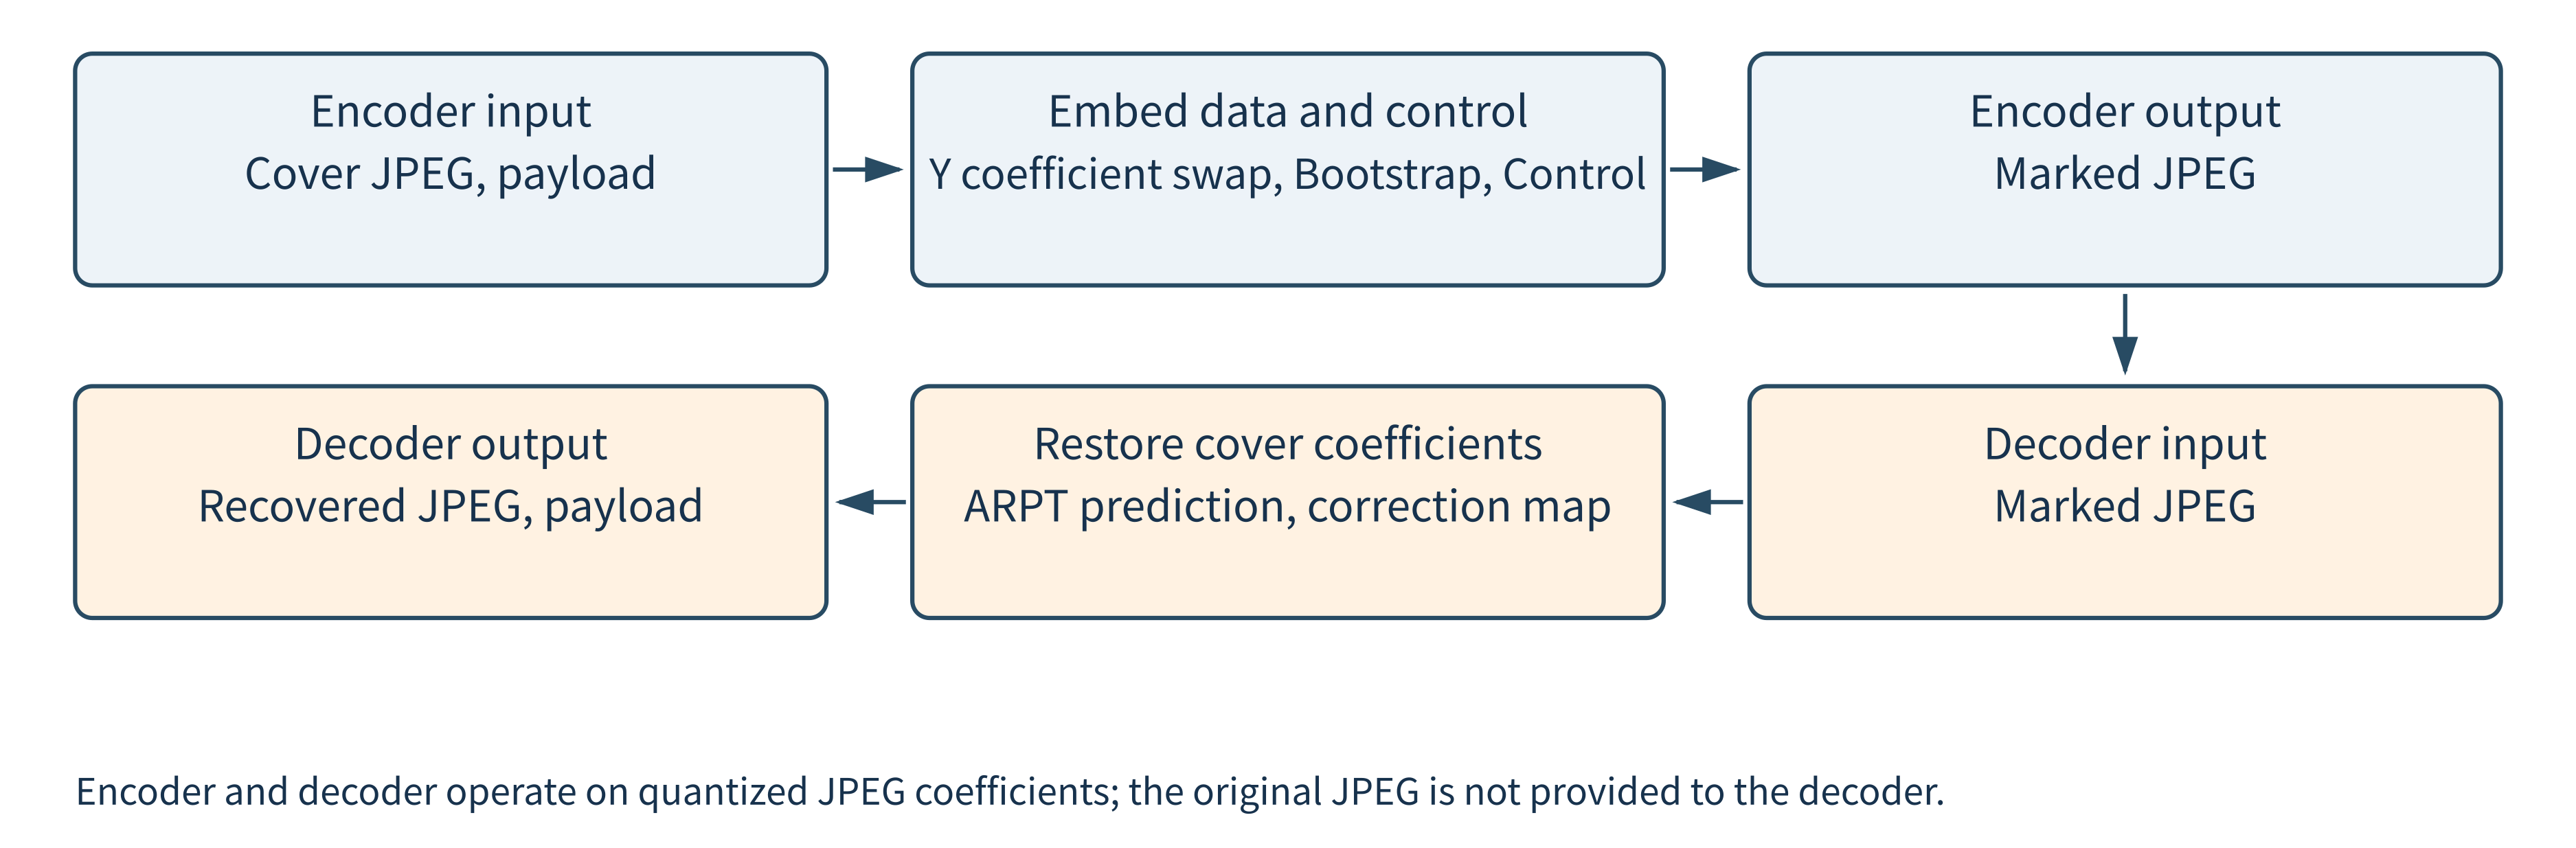
\includegraphics[width=0.95\linewidth,height=\textheight,keepaspectratio]{figures/fig1.png}

Figure 1. Self-contained encoding and decoding. The encoder stores the
message and restoration information in the same marked JPEG. The decoder
reads the message from the coefficient order, then restores the original
coefficients using swap-state predictions and the correction map.
\end{minipage}

\subsection*{2.2 Conventional baseline}\label{conventional-baseline}
\addcontentsline{toc}{subsection}{2.2 Conventional baseline}

A spatial integer-rounding heuristic is used as an external baseline
comparator. Given a quantized DCT block \(A\) and the candidate
\(B = T(A)\) obtained by swapping AC coefficients (1,4), a standard
orthonormal float32 inverse discrete cosine transform (IDCT) produces
the corresponding spatial blocks \(I_A\) and \(I_B\). The rounding
residual at pixel \((m,n)\) is defined as

\[
r[m,n] = |I[m,n] - \mathrm{round}(I[m,n])| \in [0, 0.5]. \tag{4}
\]

With the integer-proximity threshold set to \(T_{\mathrm{hr}} = 0.3\),
the number of qualifying pixels among the 64 pixels is counted:

\[
i_A = \sum_{m=0}^7 \sum_{n=0}^7 \mathbf{1}[r_A[m,n] < T_{\mathrm{hr}}], \quad i_B = \sum_{m=0}^7 \sum_{n=0}^7 \mathbf{1}[r_B[m,n] < T_{\mathrm{hr}}]. \tag{5}
\]

Unmodified natural-image blocks have more spatial pixel values close to
integers. The predicted swap state is therefore
\(\hat{s} = \mathbf{1}[i_B > i_A]\): if \(i_B > i_A\), input block \(A\)
is classified as swapped (\(\hat{s}=1\)); otherwise, if \(i_A \ge i_B\),
it is classified as unswapped (\(\hat{s}=0\)).

\subsection*{2.3 ARPT architecture and feature
construction}\label{arpt-architecture-and-feature-construction}
\addcontentsline{toc}{subsection}{2.3 ARPT architecture and feature
construction}

ARPT retains the input block as candidate A and swaps its two designated
coefficients to form candidate B. It compares these arrangements to
determine whether the input block was swapped. The model uses three
feature types, comprising 129 feature tokens. Adding one
\texttt{{[}CLS{]}} token gives an input sequence of length 130 (Figure
2).

\textbf{64 spatial tokens:} At each spatial location, the rounding
residuals of both candidates, their difference, and their sum describe
the local residual relationship:

\[
x_{\mathrm{sp},k} = [2r_{A,k}, 2r_{B,k}, 2(r_{A,k}-r_{B,k}), r_{A,k}+r_{B,k}]^\top \in \mathbb{R}^4. \tag{6}
\]

Spatial indices range from 0 to 63. The first three components are
multiplied by 2 so that the residual components lie in \([0,1]\) and
their difference in \([-1,1]\). The sum already lies in \([0,1]\) and
retains its original scale.

\textbf{49 distribution-profile tokens:} Spatial tokens retain
location-specific residual information, whereas profile tokens compare
the residual distributions of the entire block. Thresholds are set at
intervals of 0.01 from 0.01 to 0.49. For each threshold, the difference
between the numbers of residuals strictly below that threshold is scaled
by a threshold-specific standard deviation estimated from the training
data. The mean of the difference is fixed at zero, so swapping the
candidates negates the distribution-difference vector:

\[
\begin{aligned}
t_j &= 0.01j,\qquad j=1,\dots,49,\\
d_j &= \sum_{k=0}^{63} \mathbf{1}[r_{A,k} < t_j] - \sum_{k=0}^{63} \mathbf{1}[r_{B,k} < t_j], \\
z_j &= d_j / \sigma_j, \qquad x_{\mathrm{pr},j} = [z_j, (t_j-0.25)/0.24]^\top \in \mathbb{R}^2.
\end{aligned} \tag{7}
\]

The first component is the scaled residual-count difference. The second
maps the threshold coordinate to \([-1,1]\), identifying the threshold
associated with each token.

\textbf{16 coefficient-context tokens:} Zero-based zigzag indices 0
through 15, including DC, supply low-frequency coefficient information.
Both candidates are standardized using shared position-specific means
and standard deviations estimated from the training data. The
standardized coefficients, their difference, and their sum form the
features at each position:

\[
x_{\mathrm{cf},m} = [c_{A,m}, c_{B,m}, c_{A,m}-c_{B,m}, c_{A,m}+c_{B,m}]^\top \in \mathbb{R}^4,
\quad m=0,\dots,15. \tag{8}
\]

Here, \(c_{A,m}\) and \(c_{B,m}\) are the standardized coefficients of
the two candidates at zigzag position \(m\).

Each feature type is linearly projected to 64 dimensions. Learnable
position and type embeddings are added, and the tokens are combined with
the \texttt{{[}CLS{]}} token to form the input sequence. The Transformer
encoder {[}5{]} has 2 layers, 4 attention heads, and a 128-dimensional
feed-forward network, with GELU activation and dropout set to 0. The
scoring pipeline is

\textbf{Feature embedding → Transformer encoder → \texttt{{[}CLS{]}}
output → scoring head → score}

The shared scorer comprises this entire pipeline. Using the same
parameters, the model scores the original candidate order and the
reversed order, divides their score difference by 2, and applies a
sigmoid to obtain the predicted swap-state probability:

\[
f(A,B,z) = \frac{g(A,B,z)-g(B,A,-z)}{2}, \qquad p = \mathrm{sigmoid}(f)=\frac{1}{1+\exp(-f)}. \tag{9}
\]

Here, \(g\) is the shared scorer, \(z\) is the distribution-difference
vector in Eq. (7), and \(p\) is the probability that the model
classifies input block A as swapped. Reversing the candidate order
exchanges their features and negates the differences, while leaving the
sums unchanged. Consequently, the score difference \(f\) changes sign,
giving the model its antisymmetric structure. In direct classification,
a probability of at least 0.5 indicates a swapped block. At \(f=0\), the
probability is exactly 0.5 in either order; the threshold rule therefore
does not imply complementary hard labels at this tie.

\begin{minipage}{\linewidth}
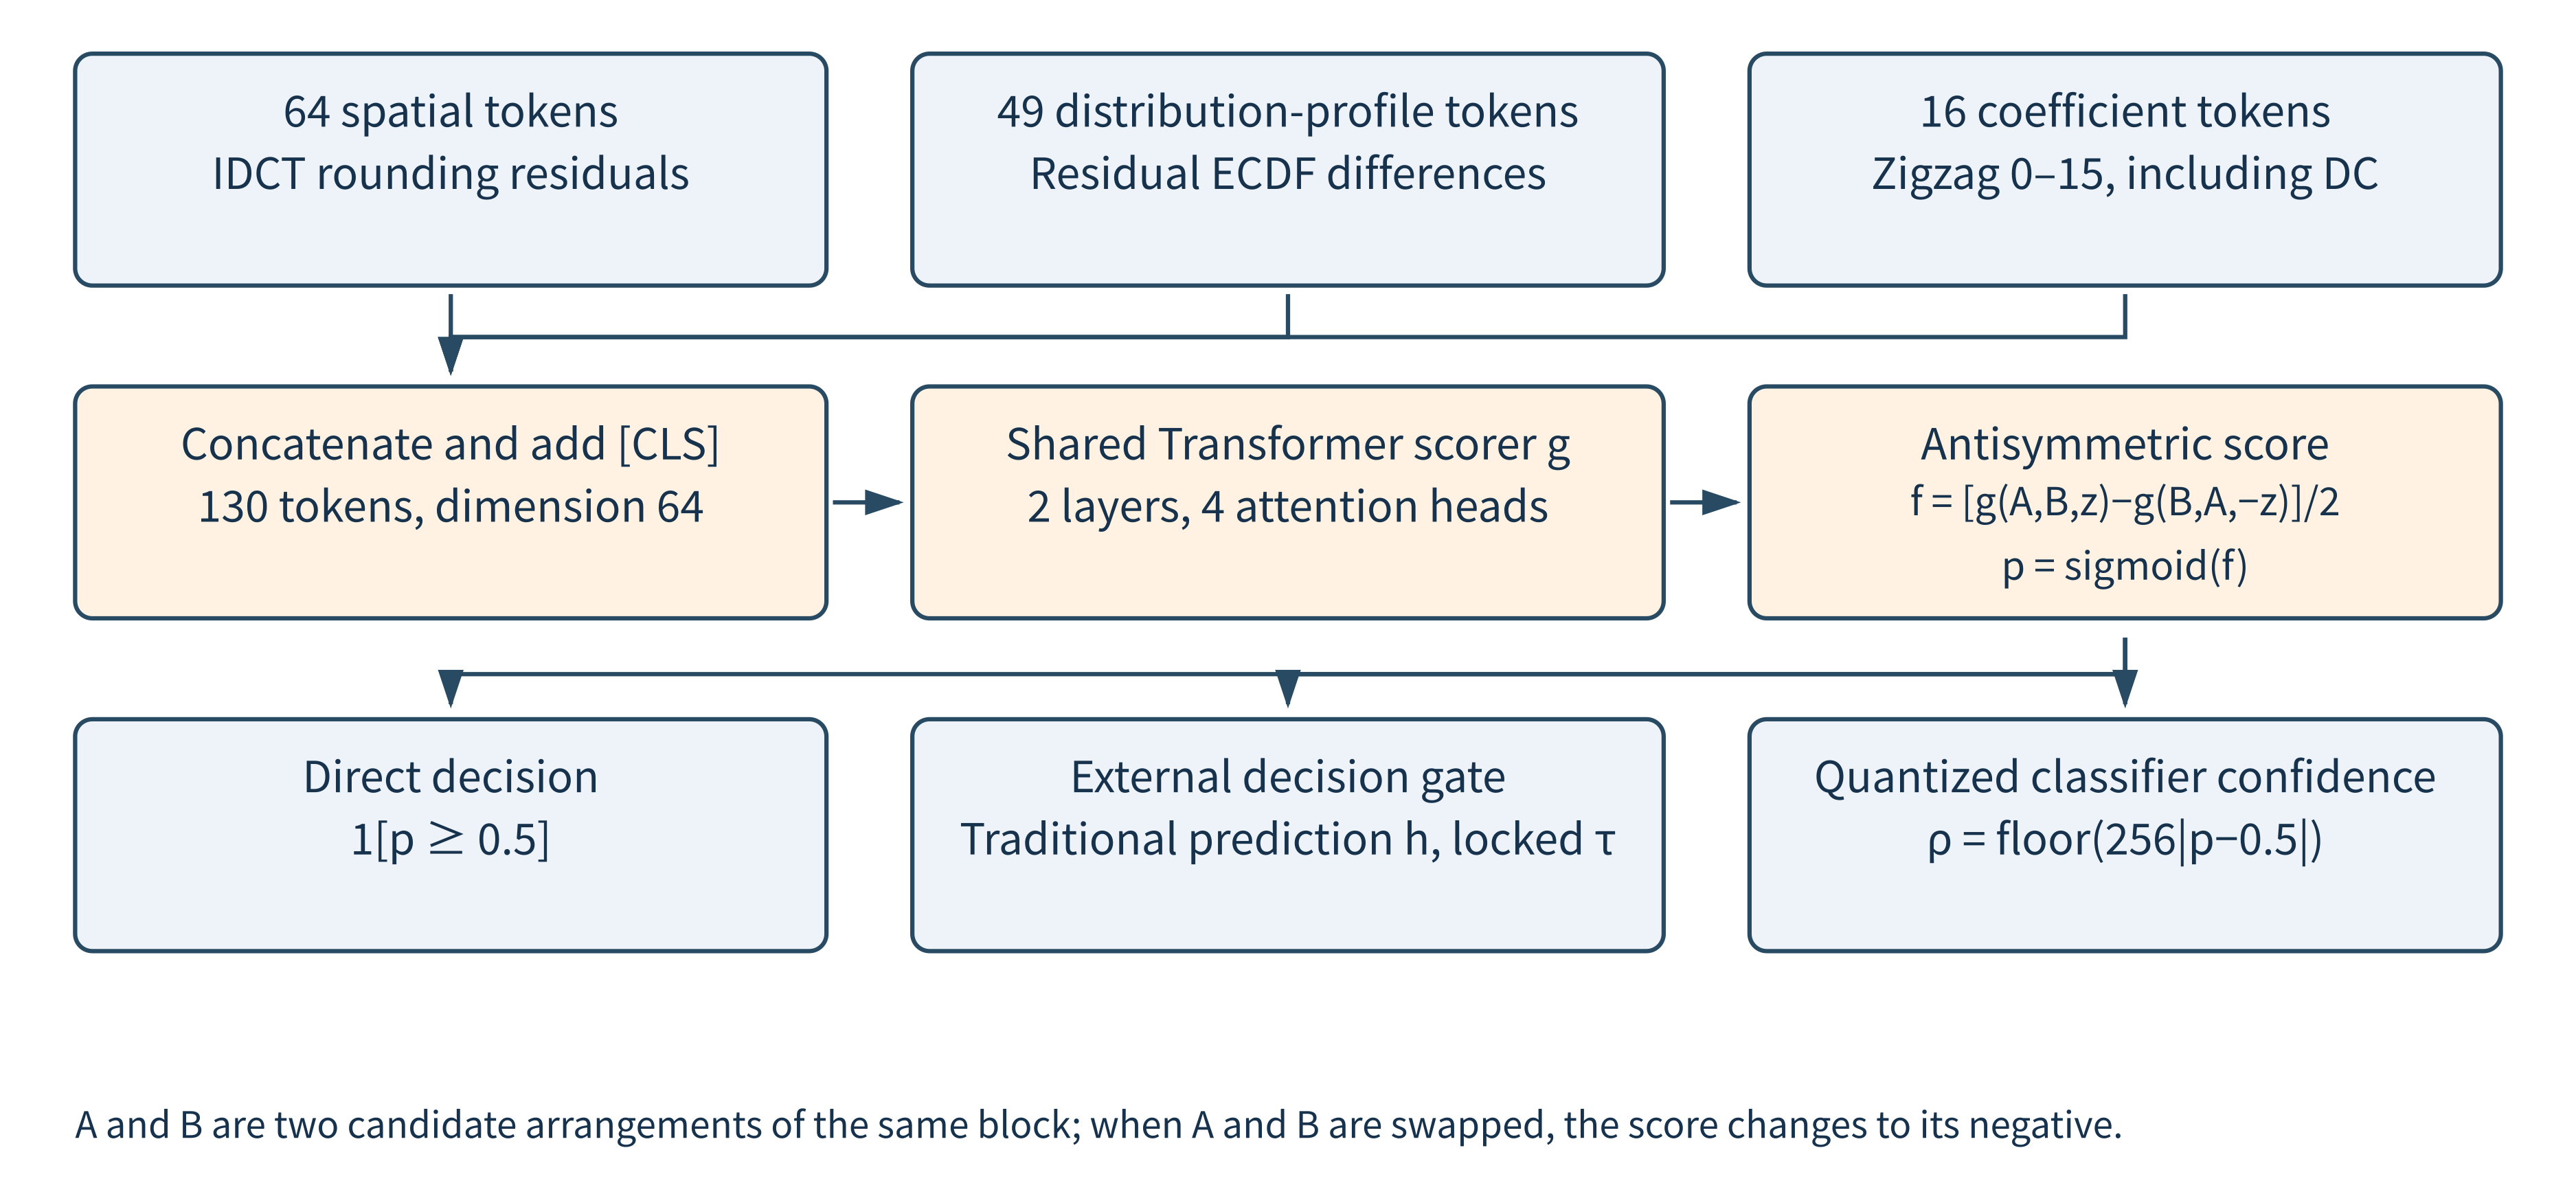
\includegraphics[width=0.95\linewidth,height=\textheight,keepaspectratio]{figures/fig2.png}

Figure 2. ARPT architecture. Three feature types are evaluated by a
shared model, and the difference between scores for the two candidate
orders produces the swap-state prediction.
\end{minipage}

ARPT has 78,657 trainable parameters and is trained with binary
cross-entropy loss without class weighting. The deployed model uses seed
2025, the AdamW optimizer {[}6{]}, a learning rate of
\(3\times10^{-4}\), weight decay of \(10^{-4}\), and a batch size of
256, for 10 epochs. The model and gating threshold are selected
according to the number of post-gating errors on the validation set. The
deployed checkpoint is epoch 10, with a threshold of 0.555.

A decision gate combines the conventional method with ARPT. The ARPT
decision replaces the conventional decision only when its probability in
support of the opposite decision reaches the specified threshold;
otherwise, the conventional decision is retained. The conventional
decision is used only at this decision stage, not as an ARPT input.

An ARPT output closer to 0 or 1 indicates greater confidence. Its
distance from 0.5 is used as the confidence score for carrier selection
in the next subsection.

\subsection*{2.4 Confidence-guided carrier
selection}\label{confidence-guided-carrier-selection}
\addcontentsline{toc}{subsection}{2.4 Confidence-guided carrier
selection}

Blocks for which the model is more confident are used first to reduce
the correction information required after misclassification. An output
\(p\) close to 0 or 1 indicates a stronger preference for one decision,
whereas an output near 0.5 indicates uncertainty. The carrier-selection
confidence score is therefore \(|p-0.5|\).

To compute confidence consistently before and after embedding, both
encoder and decoder first arrange the two designated coefficients of
every eligible block in the same order: the smaller coefficient at
position 1 and the larger at position 4. The resulting block is then
passed to ARPT. Even if embedding swaps the coefficients, this canonical
arrangement produces the same model input. To reduce the effect of small
floating-point differences on ranking, confidence is converted to an
integer:

\[
\rho = \lfloor256|p-0.5|\rfloor, \qquad \rho \in \{0, \ldots, 128\}. \tag{10}
\]

Eligible blocks are ranked in descending order of model confidence, and
the first \(K\) are selected for message embedding (Top-K selection).
Ties are resolved by an order generated from the shared key. After
selection, the message is embedded in key order: ascending coefficient
order represents 1, and descending order represents 0.

The decoder repeats the same selection procedure. To check that the
selected blocks and their order agree, the encoder stores the first 16
bytes of the carrier-list SHA-256 digest in the control packet. This
digest is used only to check selection agreement. The decoder recomputes
and compares it, and stops decoding if it does not match.

\subsection*{2.5 Self-contained protocol, restoration, and
cost}\label{self-contained-protocol-restoration-and-cost}
\addcontentsline{toc}{subsection}{2.5 Self-contained protocol,
restoration, and cost}

The Y blocks are partitioned by the shared key into three disjoint
regions (Figure 3):

\begin{itemize}
\tightlist
\item
  \textbf{Bootstrap region (25\%):} Stores a fixed 32-byte bootstrap
  packet specifying how much control information the decoder should read
  and supplying a CRC-32 checksum.
\item
  \textbf{Control region (50\%):} Stores the correction map, message
  length, correction-map encoding, and the settings and identifiers
  needed for decoding.
\item
  \textbf{Data region (25\%):} Embeds the message through coefficient
  swapping at fixed positions, here zigzag positions 1 and 4.
\end{itemize}

\begin{minipage}{\linewidth}
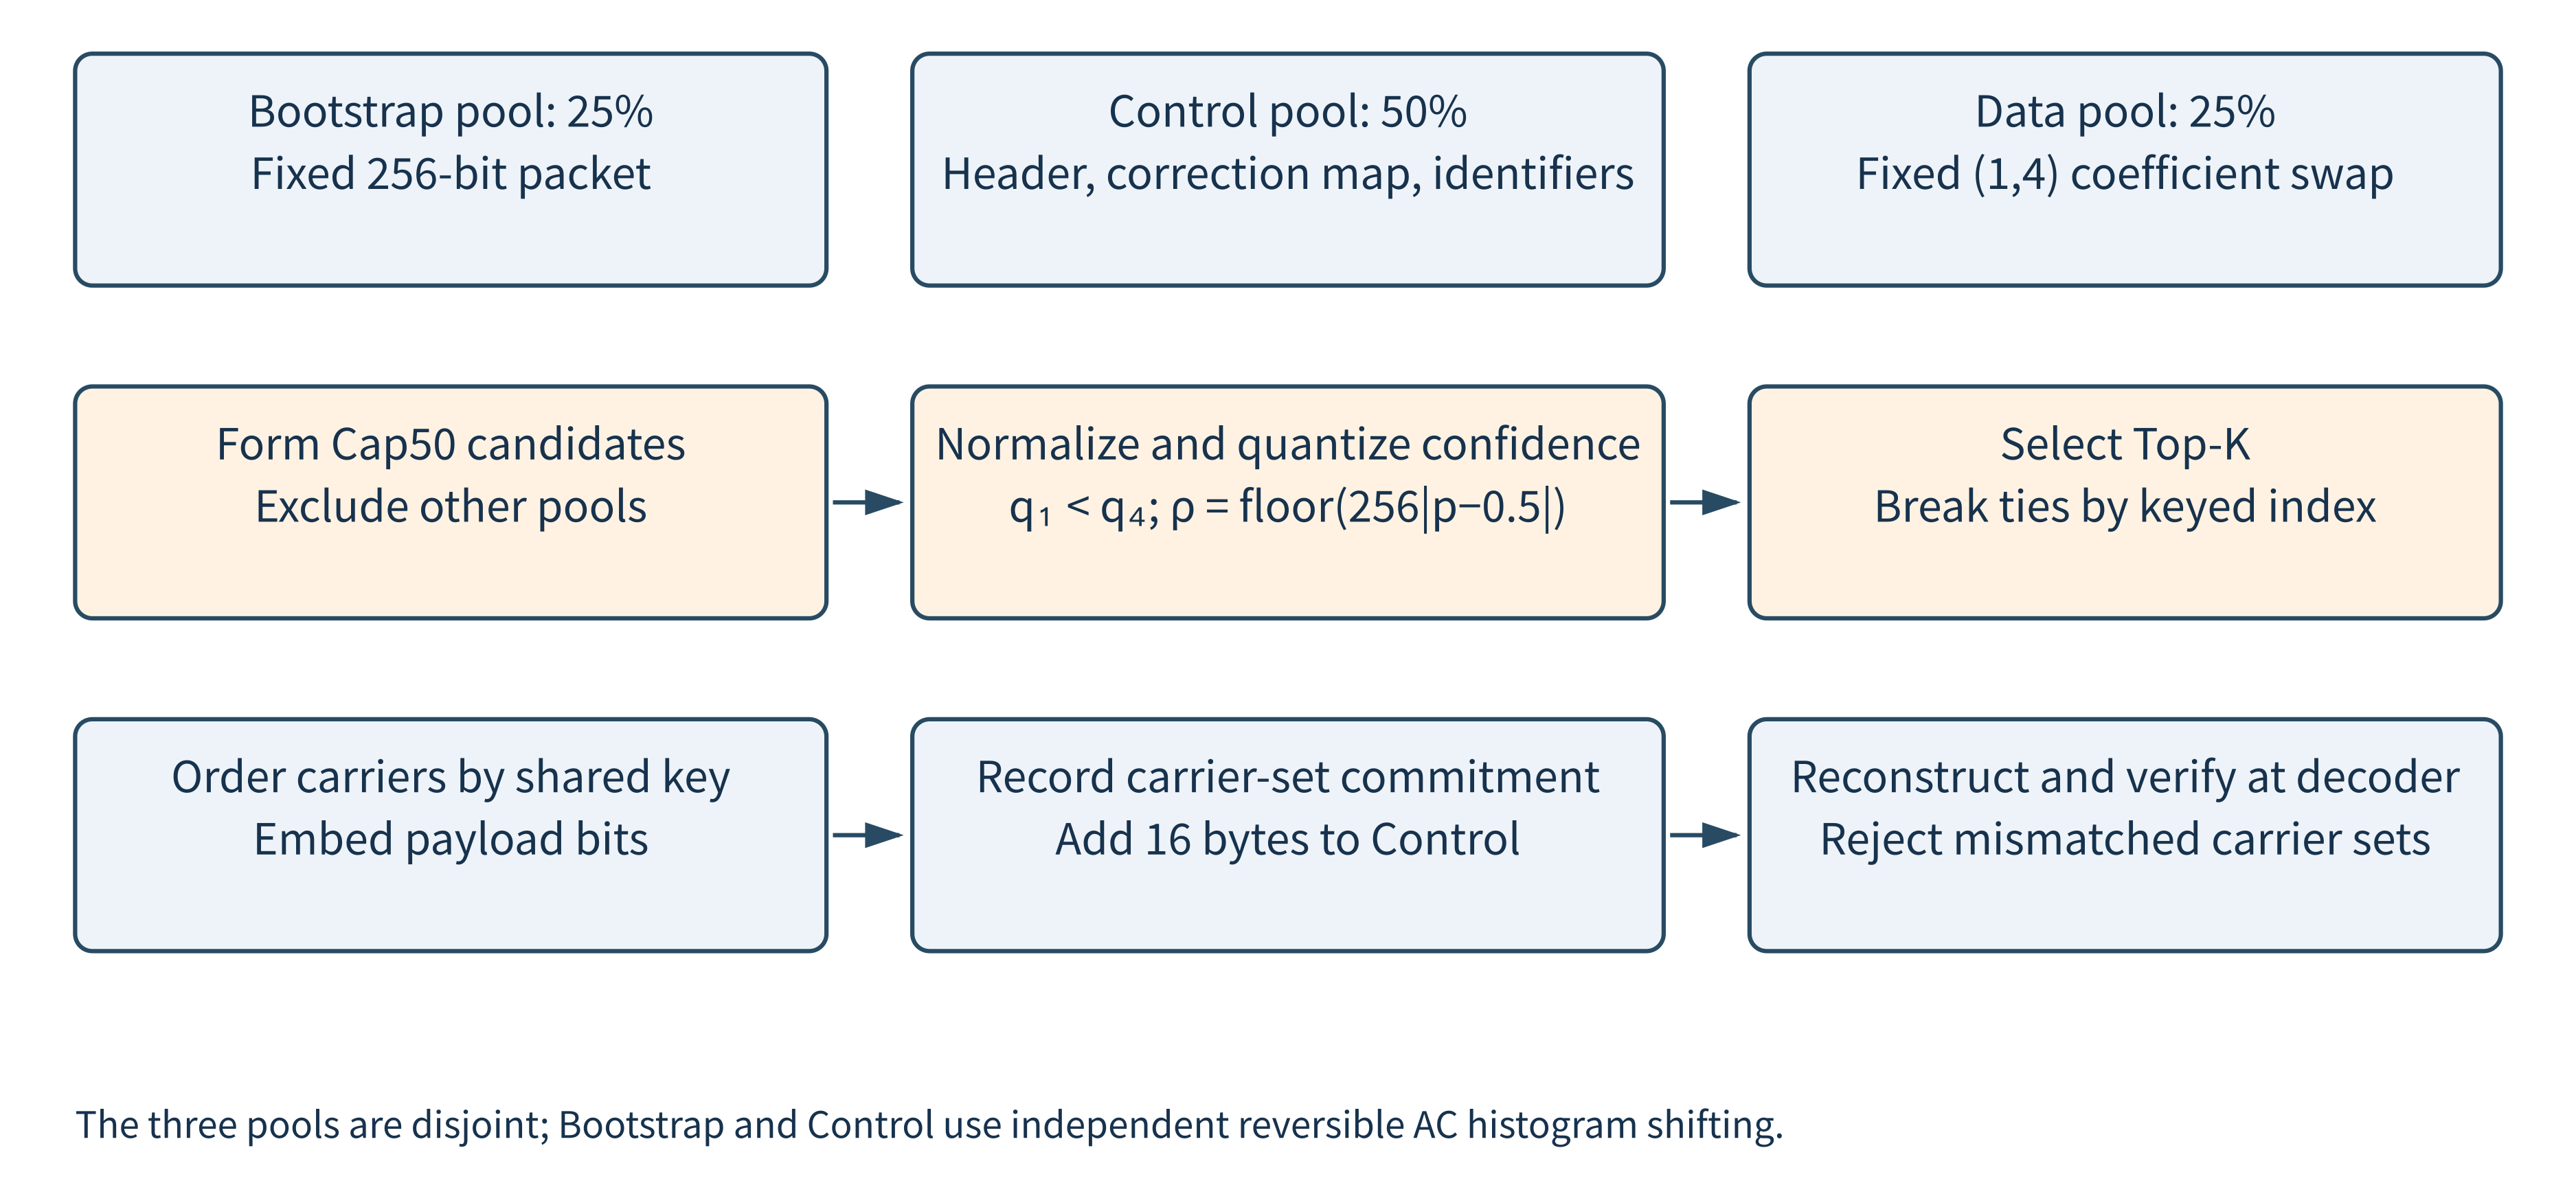
\includegraphics[width=0.95\linewidth,height=\textheight,keepaspectratio]{figures/fig3.png}

Figure 3. Three disjoint pools and confidence ranking. The bootstrap and
control pools carry information through reversible AC histogram
shifting; the data pool carries the message through coefficient
swapping.
\end{minipage}

The bootstrap and control regions store information using reversible
histogram shifting {[}7{]}. Zero coefficients are unchanged. For
coefficients equal to \(1\) or \(-1\), the magnitude represents one
message bit; other coefficients are shifted outward by one to create
space:

\[
a' = \begin{cases}
0, & a = 0, \\
\mathrm{sign}(a)(1+d), & |a| = 1, \\
a + \mathrm{sign}(a), & |a| > 1.
\end{cases} \tag{11}
\]

Here, \(a\) is the original coefficient and \(d\) is the bit, 0 or 1, to
be written. For 0, the magnitude stays at 1; for 1, it becomes 2, with
the sign unchanged. After extraction, the decoder restores coefficients
of magnitude 1 or 2 to magnitude 1 and shifts the other modified
coefficients back to their original values.

As shown in Figure 1, the decoder reads the bootstrap packet, reads the
control information, identifies the data carriers, extracts the message,
and finally restores the original coefficients using ARPT and the
correction map. Each region is read according to the length recorded in
the packet. Decoding stops if the length or format is inconsistent.

The correction map records which carriers have incorrectly predicted
swap states: 0 denotes a correct prediction, and 1 an error. If \(w\) of
the \(K\) selected carriers require correction, the correction rate is
\(w/K\).

Four lossless storage methods are compared: direct bit packing (packed),
zlib compression, storage of error positions only (sparse), and
combinatorial encoding. The encoder chooses the shortest packet and
records its encoding in the control region so that the decoder can
reconstruct the map.

Combinatorial encoding {[}8{]} records the index of the error-position
set among all possible sets of \(w\) errors in \(K\) positions. For
error positions \(0 \le a_1 < \cdots < a_w < K\), the index and required
bit count are

\[
\mathrm{rank} = \sum_{i=1}^{w}\binom{a_i}{i}, \qquad
0 \le \mathrm{rank} < \binom{K}{w}, \qquad
B_{\mathrm{rank}} = \left\lceil\log_2\binom{K}{w}\right\rceil. \tag{12}
\]

The error count \(w\) is stored separately as an unsigned LEB128
integer. With \(K\), \(w\), and the combinatorial rank, the decoder
reconstructs the error positions.

To compare overhead at the same embedded message size, overhead-adjusted
payload is defined as the actual message size \(K\) minus the sizes of
the control and bootstrap packets:

\[
P_{\mathrm{adj}} = K - B_{\mathrm{control}} - B_{\mathrm{bootstrap}}, \qquad B_{\mathrm{bootstrap}} = 256\ \text{bits}. \tag{13}
\]

The message actually written and extracted is still the \(K\) bits in
the data region. Because the bootstrap, control, and data regions are
physically disjoint pools, overhead-adjusted payload is only an
accounting metric; its increase does not constitute experimental
evidence of an increase in the maximum embeddable message size. A larger
\(P_{\mathrm{adj}}\) means less packet overhead for the same message
size. The control-packet size already includes the correction map, which
is not subtracted again.

Restoration is checked using the JPEG files actually stored. The
extracted message must match the original message, and the restored Y,
Cb, and Cr quantized coefficients and RGB pixels produced by a fixed
decoder must each be identical to their pre-embedding counterparts.
Exact restoration is declared only when all three checks pass.

\subsection*{2.6 Data and comparison
design}\label{data-and-comparison-design}
\addcontentsline{toc}{subsection}{2.6 Data and comparison design}

The study uses 37 iPhone 14 Pro images, with 2,000 coefficient pairs
constructed per image, for 74,000 pairs. Each pair has an unswapped and
a swapped state, yielding 148,000 samples labeled 0 and 1, respectively.

The data are split by image into 25 training images, 6 validation
images, and 6 test images, with no overlap between the three sets.

The main comparison fixes the embedded message at 2,560 bytes, or
\(K=20,480\) bits, and evaluates three methods:

\begin{itemize}
\tightlist
\item
  \textbf{Conventional method:} Selects blocks in a key-generated
  pseudorandom order and predicts swap states using the conventional
  comparator.
\item
  \textbf{Keyed ARPT:} Selects blocks in the same key-generated
  pseudorandom order and predicts swap states using gated ARPT.
\item
  \textbf{Confidence-guided ARPT:} Uses the same gated ARPT predictor
  but prioritizes blocks with higher model confidence.
\end{itemize}

The first two methods isolate the difference between predictors; the
latter two isolate the effect of confidence ranking. All three use the
same correction-map encoding selection procedure, and the cost of each
method's control packet is included. A separate comparison between the
conventional method and gated ARPT uses an earlier encoding
configuration; its results are reported separately.

A further 32 images from the same device are used for capacity analysis,
and 24 JPEG images and 100 DIV2K images {[}9{]} are used for stress
testing. None of these images is used for training or validation. All
are converted to JPEG with the same unit quantization tables and 4:4:4
format.

The original target for each of the 32 images was 2,560 bytes. Some
images had too few eligible blocks, so the message size was subsequently
adjusted to the available block count, with a maximum of 2,560 bytes:

\[
L_i = \min(2560, \lfloor N_i/8\rfloor)\ \text{bytes}, \qquad K_i = 8L_i. \tag{14}
\]

Here, \(N_i\) is the number of eligible blocks in the data region of
image \(i\), and \(L_i\) is the embeddable byte count. This adjustment
was made after the original capacity failures, and the results are
reported as a post hoc analysis.

Per-image gain is the difference in overhead-adjusted payload between
ARPT and the conventional method. Paired bootstrap resampling at the
image level estimates the 95\% confidence interval for the mean gain.
For the 24 images that succeeded at the fixed message size, the original
results from 10,000 resamples with random seed 2025 are retained. For
the 32 capacity-adjusted images, 100,000 resamples are used with random
seed 20260918.

The correction-map encoding experiment uses the six validation images.
The same map from each image is encoded by all four methods and compared
with automatic selection, recording the required bit counts.

\section*{3. Experimental results}\label{experimental-results}
\addcontentsline{toc}{section}{3. Experimental results}

\subsection*{3.1 Marked images and swap-state
classification}\label{marked-images-and-swap-state-classification}
\addcontentsline{toc}{subsection}{3.1 Marked images and swap-state
classification}

Figure 4 shows three watermarked JPEG images. Confidence-guided ARPT
selects the blocks in each image. The left and right images each carry
2,560 bytes, and the middle image carries 2,448 bytes.

\begin{minipage}{\linewidth}
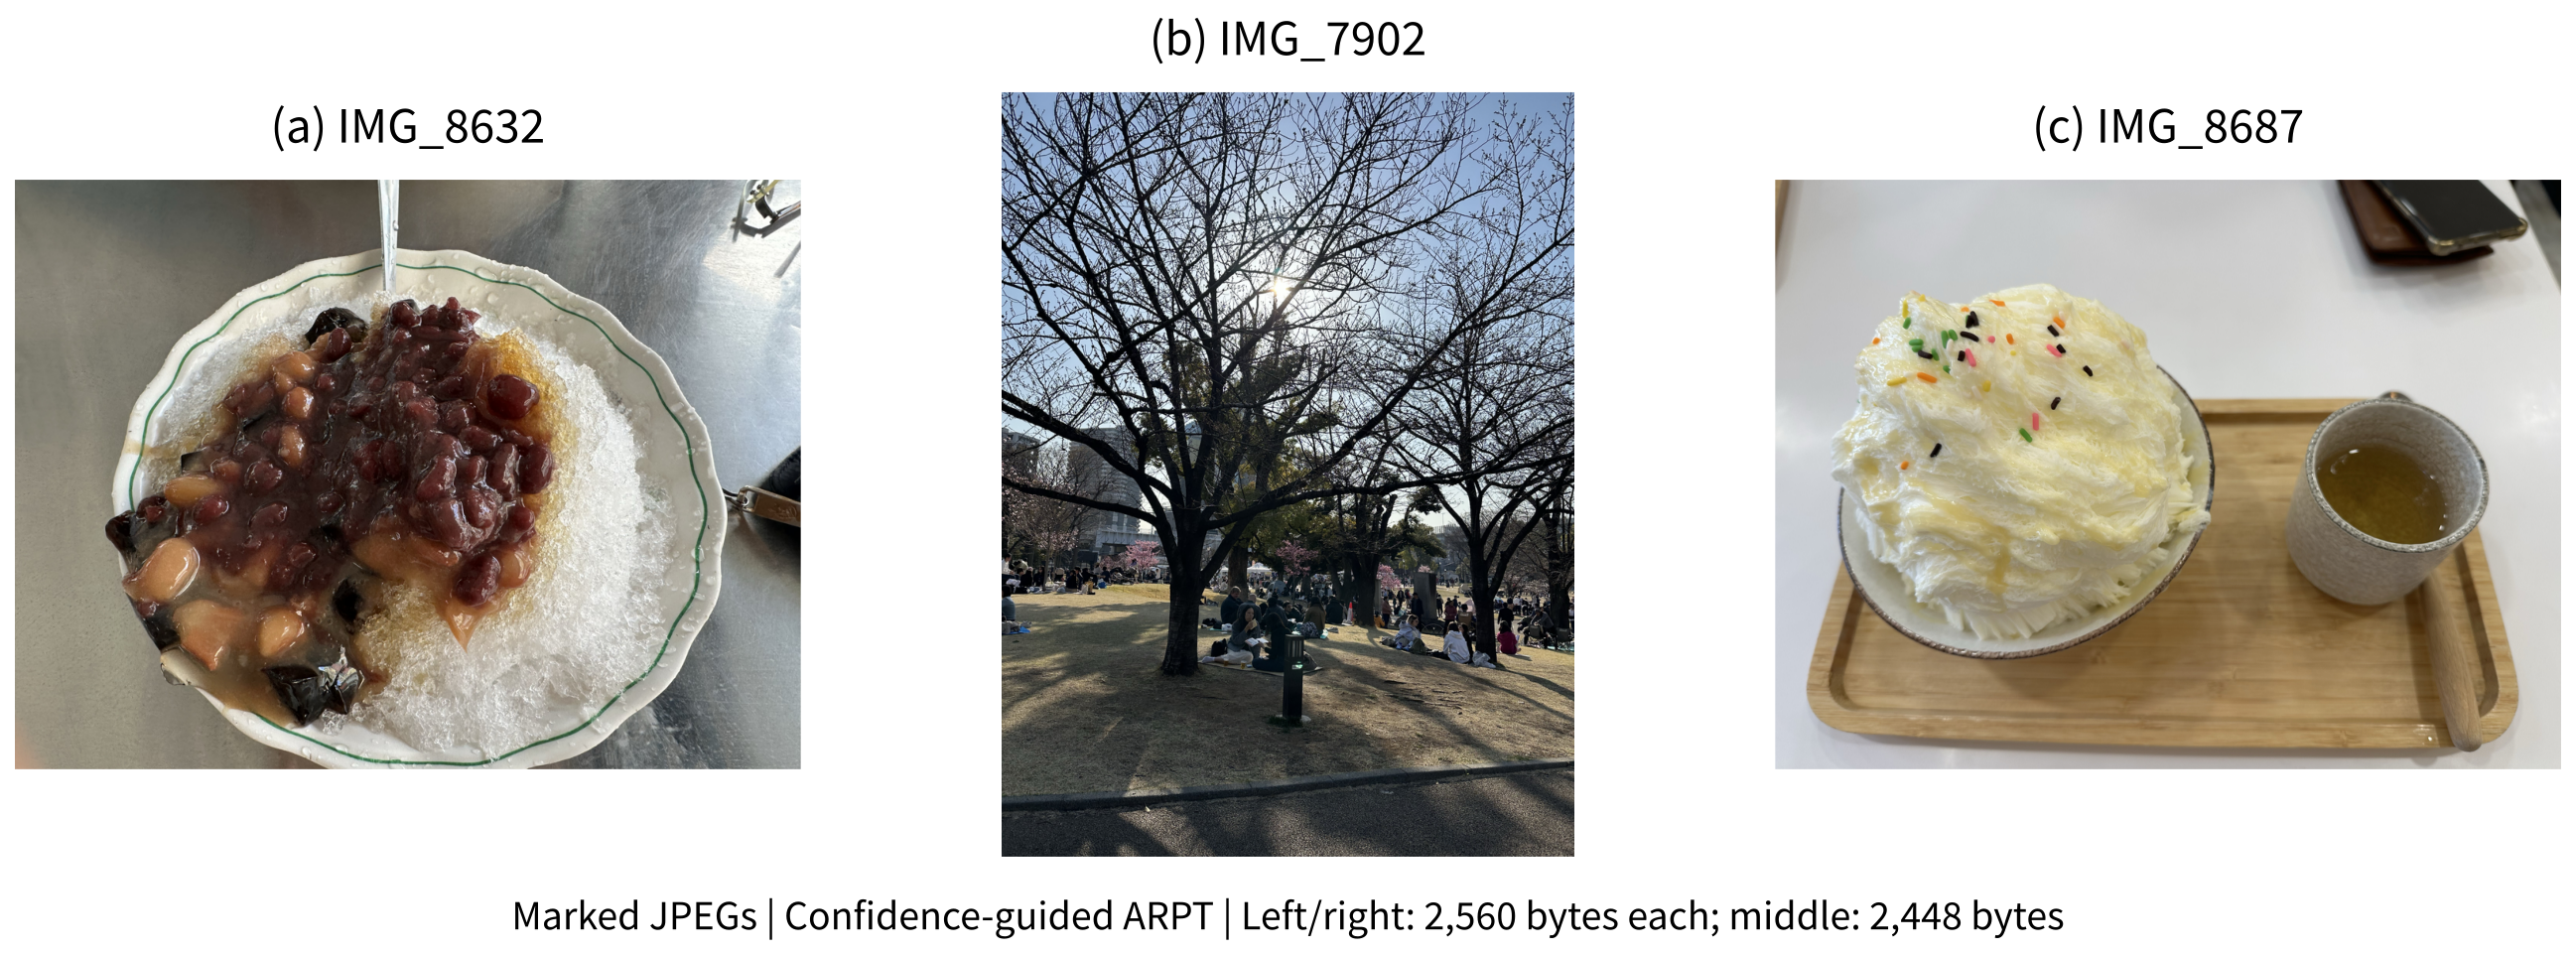
\includegraphics[width=0.95\linewidth,height=\textheight,keepaspectratio]{figures/fig4.png}

Figure 4. Three watermarked JPEG images. The left and right images each
carry a 2,560-byte message; the middle image carries a 2,448-byte
message.
\end{minipage}

Swap-state classification is evaluated on 12,000 coefficient pairs from
the six test images. Both the unswapped and swapped states are tested
for every pair, giving 24,000 decisions.

The conventional method achieves 91.17\% accuracy, with 2,119 errors.
Direct ARPT classification achieves a mean accuracy of 94.66\% over
three training seeds, with a mean of 1,282 errors, 837 fewer than the
conventional method.

Gated ARPT combines the conventional decision with the model prediction:
it retains the conventional decision unless ARPT's confidence in the
opposite decision reaches the specified threshold. Over the three seeds,
its mean accuracy is 94.62\%, with a mean of 1,291 errors.

Direct ARPT outperforms the conventional method for all three seeds, but
gating does not consistently improve the result. Subsequent
carrier-selection and encoding--decoding experiments use the seed-2025
model with the gating threshold selected on the validation data.

\begin{minipage}{\linewidth}
Table 1. Swap-state classification on the test set.

{\def\LTcaptype{none} % do not increment counter
\begin{longtable}[]{@{}lrrrr@{}}
\toprule\noalign{}
Seed & Direct ARPT accuracy & Errors & Gated ARPT accuracy & Errors \\
\midrule\noalign{}
\endhead
\bottomrule\noalign{}
\endlastfoot
2025 & 94.71\% & 1,270 & 94.76\% & 1,258 \\
2026 & 94.55\% & 1,308 & 94.53\% & 1,313 \\
2027 & 94.72\% & 1,268 & 94.58\% & 1,302 \\
Mean & 94.66\% & 1,282 & 94.62\% & 1,291 \\
\end{longtable}
}
\end{minipage}

\subsection*{3.2 Carrier selection and restoration cost on the test
set}\label{carrier-selection-and-restoration-cost-on-the-test-set}
\addcontentsline{toc}{subsection}{3.2 Carrier selection and restoration
cost on the test set}

The conventional method, Keyed ARPT, and confidence-guided ARPT are
compared on the six test images. Each method embeds 2,560 bytes per
image, with \(K=20,480\) bits fixed.

The conventional method and Keyed ARPT select the same blocks, with
selected-carrier error rates of 8.77\% and 5.45\%, respectively. With
the same gated ARPT predictor, confidence-guided selection further
reduces the error rate to 0.66\% (Figure 5). The mean numbers of blocks
requiring correction per image are 1,795.17, 1,116.33, and 134.50,
respectively.

\begin{minipage}{\linewidth}
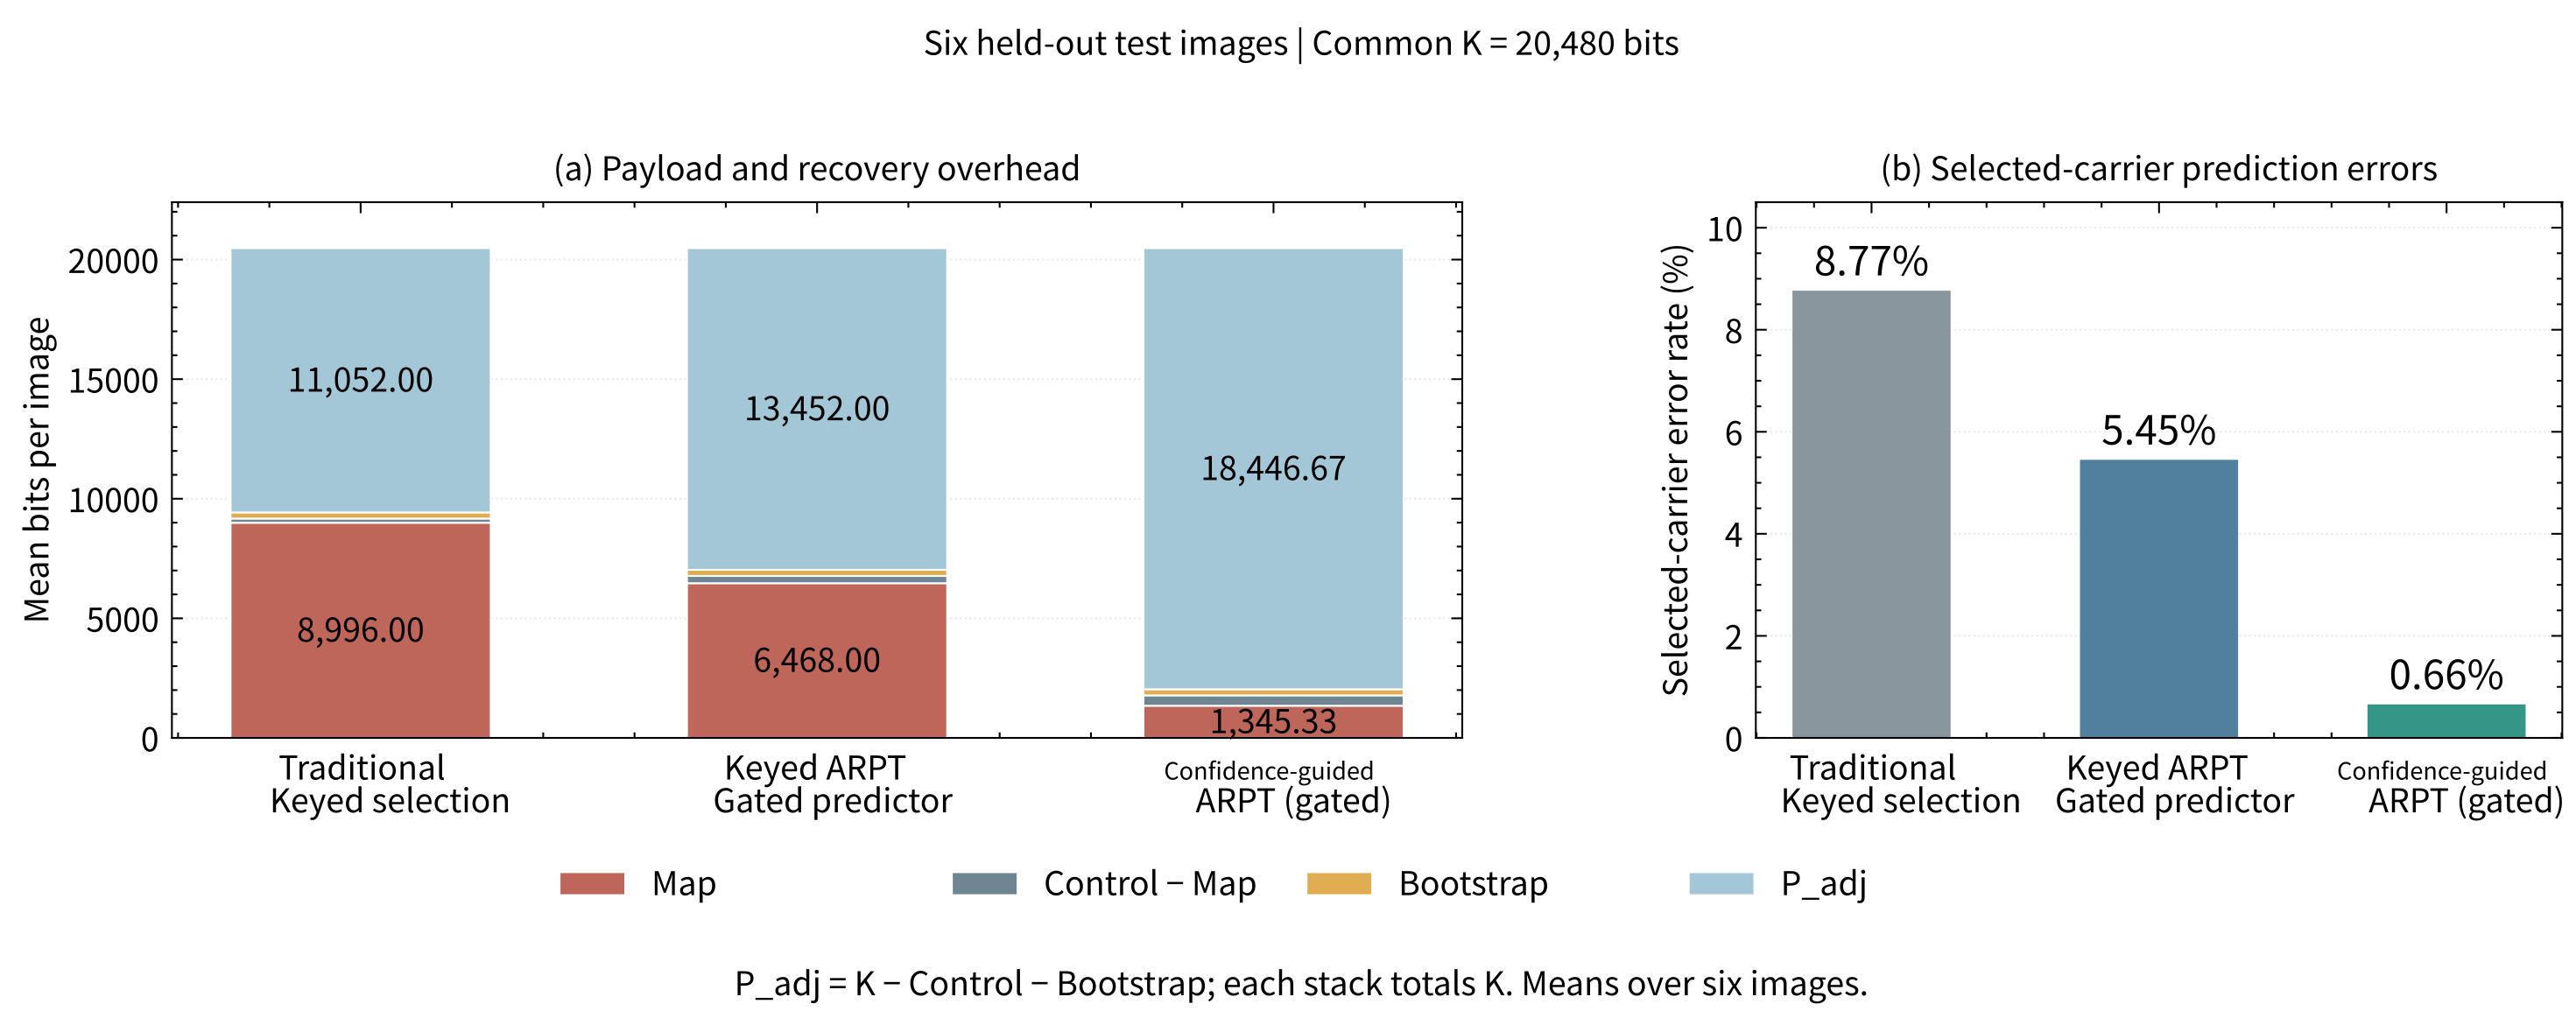
\includegraphics[width=0.95\linewidth,height=\textheight,keepaspectratio]{figures/fig5.png}

Figure 5. Carrier-selection results and restoration-information costs
for the six test images. All three methods embed 20,480 bits per image.
Values are means over the six images.
\end{minipage}

As Table 2 shows, the mean correction-map size falls from 6,468.00 bits
for Keyed ARPT to 1,345.33 bits for confidence-guided ARPT, a reduction
of 5,122.67 bits per image. Confidence-guided selection additionally
stores a 128-bit carrier-list digest. Even with this cost included, the
control packet decreases from 6,772.00 to 1,777.33 bits.

\begin{minipage}{\linewidth}
Table 2. Mean restoration-information costs and exact-restoration
results for the six test images.

{\def\LTcaptype{none} % do not increment counter
\begin{longtable}[]{@{}lrrr@{}}
\toprule\noalign{}
Metric & Conventional method & Keyed ARPT & Confidence-guided ARPT \\
\midrule\noalign{}
\endhead
\bottomrule\noalign{}
\endlastfoot
Correction-map size (bits) & 8,996.00 & 6,468.00 & 1,345.33 \\
Control-packet size (bits) & 9,172.00 & 6,772.00 & 1,777.33 \\
Overhead-adjusted payload (bits) & 11,052.00 & 13,452.00 & 18,446.67 \\
Exact-restoration cases & 6/6 & 6/6 & 6/6 \\
\end{longtable}
}
\end{minipage}

All three methods embed 20,480 bits per image. The bootstrap packet is
256 bits, and the control packet includes the correction map.

Relative to Keyed ARPT, confidence-guided selection increases mean
overhead-adjusted payload by 4,994.67 bits. All 18 encoding--decoding
cases for the three methods recover the original message and restore
exactly the same Y, Cb, and Cr quantized coefficients and decoded RGB
pixels as before embedding.

\subsection*{3.3 Correction-map encoding}\label{correction-map-encoding}
\addcontentsline{toc}{subsection}{3.3 Correction-map encoding}

The same correction map from each of the six validation images is
encoded by different methods to compare storage requirements.

Table 3 shows that combinatorial encoding has the smallest mean
correction-map size, 1,938.67 bits.

\begin{minipage}{\linewidth}
Table 3. Mean costs of correction-map encodings on the six validation
images.

{\def\LTcaptype{none} % do not increment counter
\begin{longtable}[]{@{}
  >{\raggedright\arraybackslash}p{(\linewidth - 6\tabcolsep) * \real{0.2500}}
  >{\raggedleft\arraybackslash}p{(\linewidth - 6\tabcolsep) * \real{0.2500}}
  >{\raggedleft\arraybackslash}p{(\linewidth - 6\tabcolsep) * \real{0.2500}}
  >{\raggedleft\arraybackslash}p{(\linewidth - 6\tabcolsep) * \real{0.2500}}@{}}
\toprule\noalign{}
\begin{minipage}[b]{\linewidth}\raggedright
Encoding
\end{minipage} & \begin{minipage}[b]{\linewidth}\raggedleft
Correction-map size (bits)
\end{minipage} & \begin{minipage}[b]{\linewidth}\raggedleft
Control-packet size (bits)
\end{minipage} & \begin{minipage}[b]{\linewidth}\raggedleft
Overhead-adjusted payload (bits)
\end{minipage} \\
\midrule\noalign{}
\endhead
\bottomrule\noalign{}
\endlastfoot
packed & 20,688.00 & 21,120.00 & −896.00 \\
zlib & 2,926.67 & 3,358.67 & 16,865.33 \\
sparse & 2,373.33 & 2,805.33 & 17,418.67 \\
combinatorial & 1,938.67 & 2,370.67 & 17,853.33 \\
Automatic encoding (new-auto) & 1,938.67 & 2,370.67 & 17,853.33 \\
\end{longtable}
}
\end{minipage}

Automatic selection (new-auto) compares packet sizes and chooses the
shortest encoding. All six images select combinatorial encoding in this
experiment, so the results are identical. The total overhead of packed
encoding exceeds the embedded message size, and it is not selected as
the final encoding.

Five methods are tested on each of the six images, for 30
encoding--decoding cases. All recover the message and exactly restore
the original quantized coefficients and decoded RGB pixels.

\subsection*{3.4 Fixed message size and capacity
adjustment}\label{fixed-message-size-and-capacity-adjustment}
\addcontentsline{toc}{subsection}{3.4 Fixed message size and capacity
adjustment}

The conventional method and gated ARPT are compared on a further 32 JPEG
images from the same device. Automatic correction-map encoding
(legacy-auto) selects the shortest encoded packet.

The original target was 2,560 bytes per image, but 8 images had too few
eligible blocks to accommodate this message, so the goal of success on
every image was not met. For the remaining 24 images, both methods
achieve exact restoration in all 48 encoding--decoding cases. Gated ARPT
increases mean overhead-adjusted payload by 2,539.33 bits per image,
with a 95\% confidence interval of 2,329.33--2,777.01 bits.

To handle insufficient block counts, the message size is subsequently
adjusted using Eq. (14): images with enough available blocks still carry
2,560 bytes, whereas the others carry the amount they can accommodate.
Actual embedded messages range from 2,139 to 2,560 bytes, with a mean of
2,491.69 bytes. Both methods recover the message and exactly restore the
image in all 64 cases over the 32 images.

Figure 6 shows the per-image gains after message-size adjustment. Gated
ARPT increases mean overhead-adjusted payload by 2,363.25 bits per
image, with a 95\% confidence interval of 2,168.75--2,576.00 bits. The
gain is positive for all 32 images.

\begin{minipage}{\linewidth}
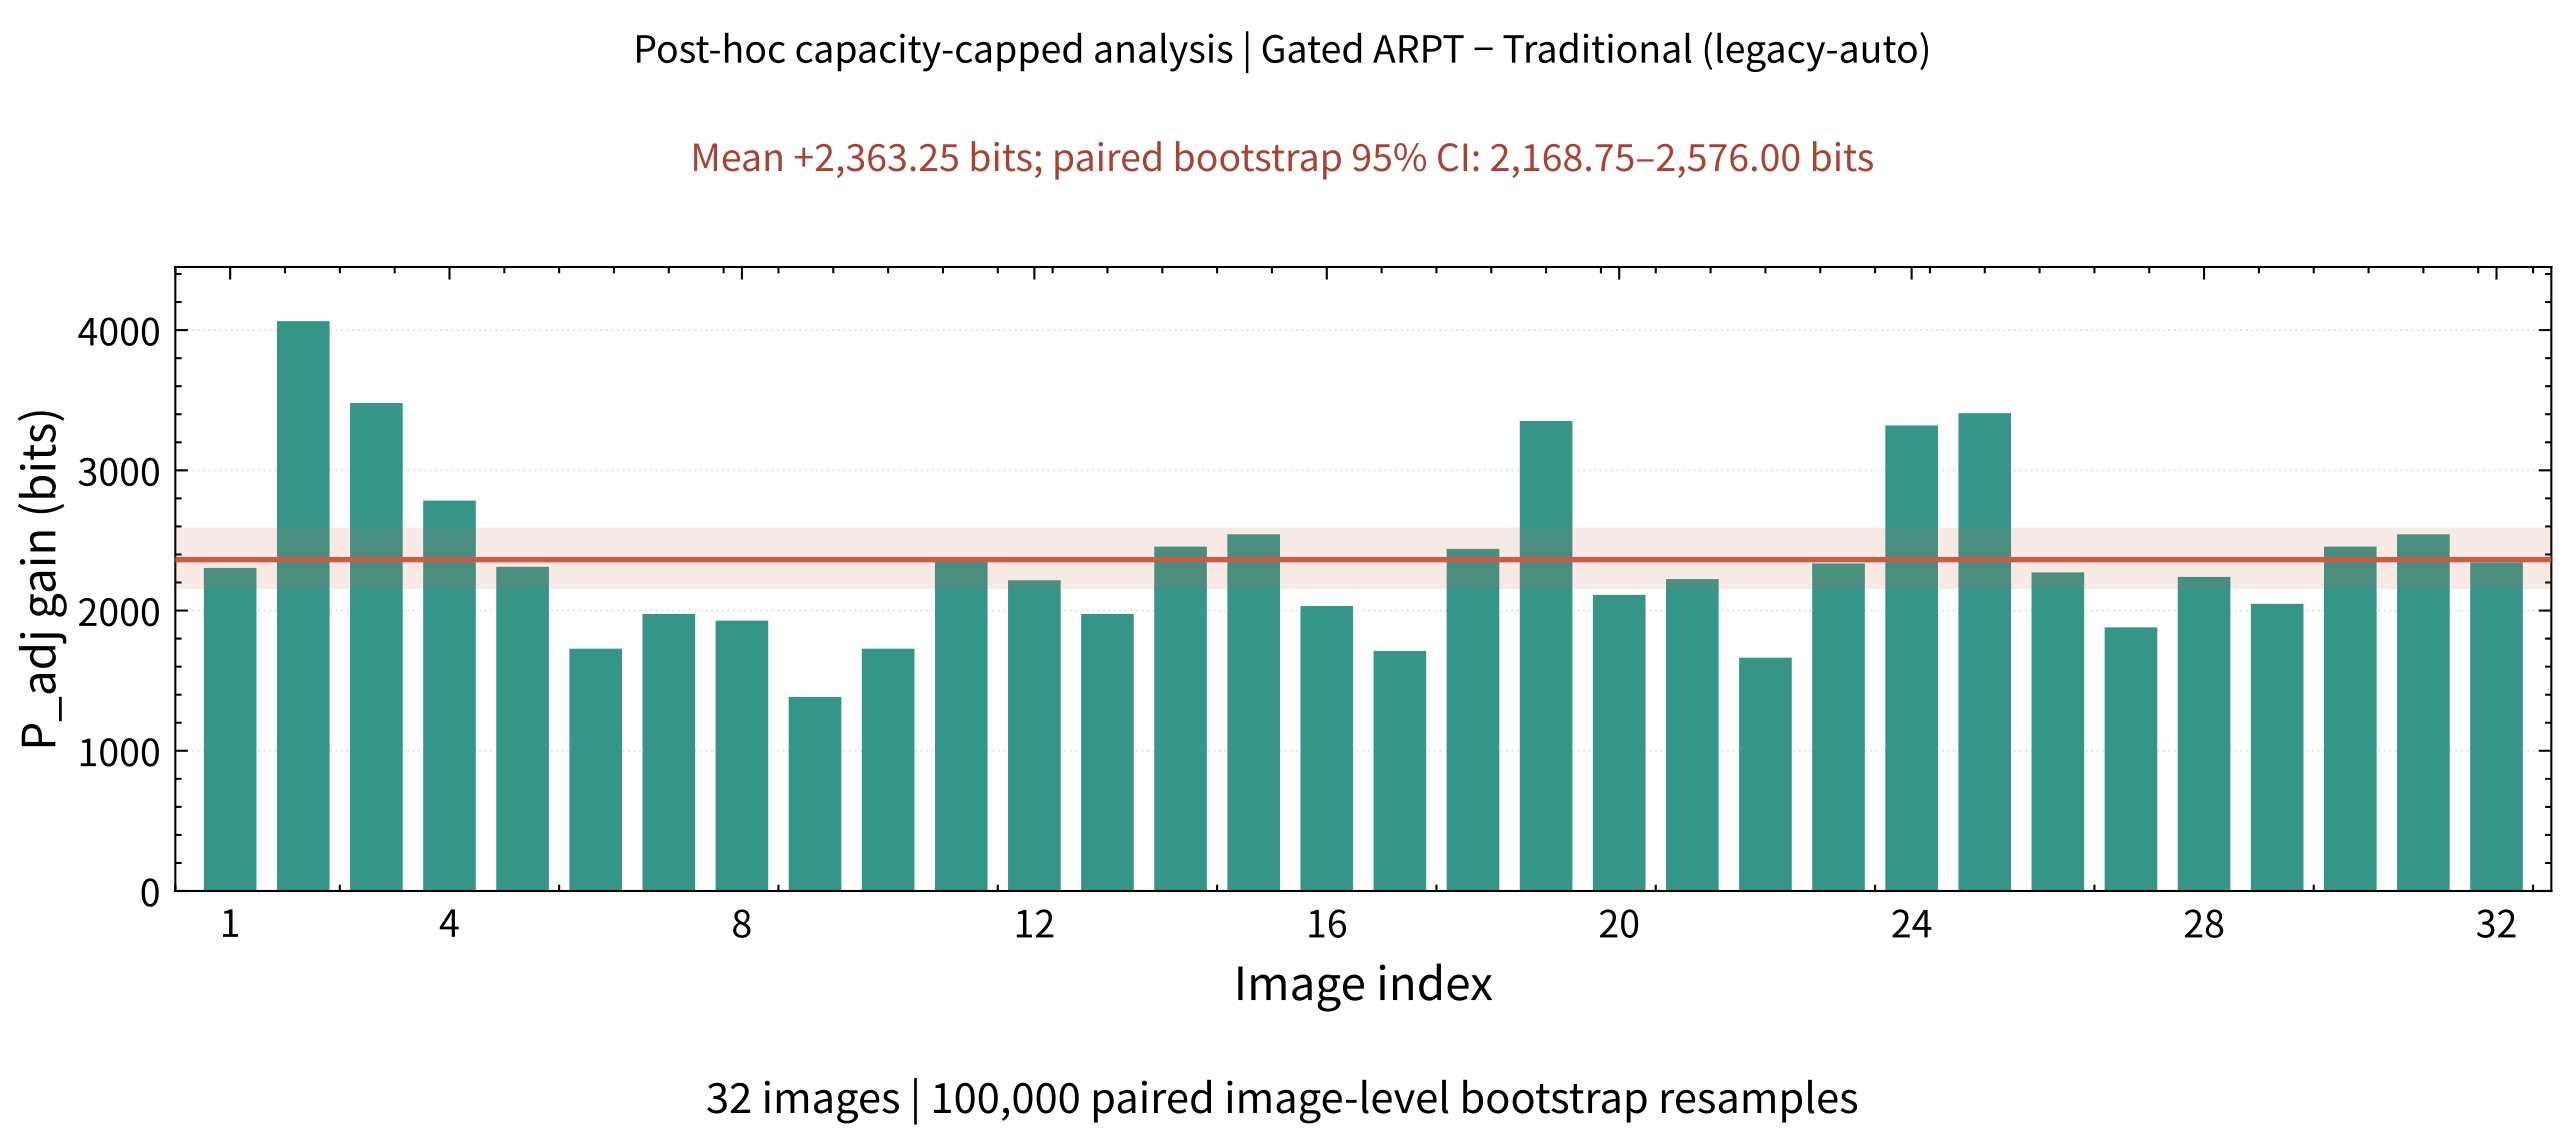
\includegraphics[width=0.95\linewidth,height=\textheight,keepaspectratio]{figures/fig6.png}

Figure 6. Per-image gains of gated ARPT over the conventional method
after message-size adjustment. The red line indicates the mean gain of
2,363.25 bits; the shaded band indicates the 95\% confidence interval
for the mean gain.
\end{minipage}

\subsection*{3.5 Tests on different image
content}\label{tests-on-different-image-content}
\addcontentsline{toc}{subsection}{3.5 Tests on different image content}

The conventional method and confidence-guided ARPT are compared on 32
outdoor JPEG images, 24 indoor JPEG images, and 100 DIV2K images.

Both methods use automatic encoding (new-auto), and the message size for
each image is set by Eq. (14). Confidence-guided ARPT uses the gated
predictor and selects carriers by model confidence.

As Table 4 shows, mean overhead-adjusted payload increases in all three
image sets. Mean gains per image are 5,288.50 bits for the 32 outdoor
JPEG images, 2,918.00 bits for the 24 indoor JPEG images, and 461.92
bits for DIV2K.

\begin{minipage}{\linewidth}
Table 4. Mean overhead-adjusted payload and exact-restoration results
for different image sets.

{\def\LTcaptype{none} % do not increment counter
\begin{longtable}[]{@{}
  >{\raggedright\arraybackslash}p{(\linewidth - 8\tabcolsep) * \real{0.2000}}
  >{\raggedleft\arraybackslash}p{(\linewidth - 8\tabcolsep) * \real{0.2000}}
  >{\raggedleft\arraybackslash}p{(\linewidth - 8\tabcolsep) * \real{0.2000}}
  >{\raggedleft\arraybackslash}p{(\linewidth - 8\tabcolsep) * \real{0.2000}}
  >{\raggedleft\arraybackslash}p{(\linewidth - 8\tabcolsep) * \real{0.2000}}@{}}
\toprule\noalign{}
\begin{minipage}[b]{\linewidth}\raggedright
Image set
\end{minipage} & \begin{minipage}[b]{\linewidth}\raggedleft
Conventional method (bits/image)
\end{minipage} & \begin{minipage}[b]{\linewidth}\raggedleft
Confidence-guided ARPT (bits/image)
\end{minipage} & \begin{minipage}[b]{\linewidth}\raggedleft
Mean gain (bits/image)
\end{minipage} & \begin{minipage}[b]{\linewidth}\raggedleft
Exact-restoration cases
\end{minipage} \\
\midrule\noalign{}
\endhead
\bottomrule\noalign{}
\endlastfoot
Outdoor JPEG, 32 images & 10,803.00 & 16,091.50 & 5,288.50 & 64/64 \\
Indoor JPEG, 24 images & 16,415.67 & 19,333.67 & 2,918.00 & 48/48 \\
DIV2K, 100 images & 2,383.28 & 2,845.20 & 461.92 & 200/200 \\
\end{longtable}
}
\end{minipage}

The indoor and outdoor photographs from the same device are
predominantly 4032×3024, approximately 12 megapixels. The DIV2K images
all have a long side of 2040 pixels and average approximately 2.84
megapixels. Because the DIV2K images are smaller, fewer blocks are
available for embedding, and the actual embedded messages are smaller.

All 312 encoding--decoding cases across the three sets recover the
message and exactly restore the original quantized coefficients and
decoded RGB pixels.

Actual embedded messages in DIV2K range from 107 to 1,227 bytes per
image, with a mean of 696.46 bytes. Overhead-adjusted payload increases
for 98 of the 100 images; for the other two, it decreases by 16 and 112
bits. A possible explanation is that the correction-map savings do not
offset the additional model and carrier-check information.

\section*{4. Conclusions and future
directions}\label{conclusions-and-future-directions}
\addcontentsline{toc}{section}{4. Conclusions and future directions}

This study proposes ARPT and confidence-guided carrier selection to
reduce restoration-information costs in reversible JPEG watermarking.
ARPT compares two candidate block arrangements and uses residual and
low-frequency coefficient features to classify the swap state.
Confidence-guided selection prioritizes blocks for which the model is
more confident, reducing the correction information that must be stored.
Remaining errors are recorded in a correction map in the same marked
JPEG, allowing the decoder to restore the original image.

On the six test images, direct ARPT achieves a mean classification
accuracy of 94.66\%, compared with 91.17\% for the conventional method.
With the same predictor and fixed message size, confidence-guided
selection reduces the selected-carrier error rate from 5.45\% to 0.66\%
and increases mean overhead-adjusted payload from 13,452.00 to 18,446.67
bits. All 18 encoding--decoding cases for the three methods recover the
message and exactly restore the original quantized coefficients and
decoded RGB pixels.

Tests on indoor, outdoor, and DIV2K images also show lower mean
restoration-information costs. The message size an image can accommodate
still depends on its eligible block count, however. At a fixed target of
2,560 bytes, some images fail because there are too few blocks; complete
encoding, decoding, and restoration are achieved only after adjusting
the message size to the available blocks. We also tested selecting fewer
blocks, adding an error-risk selector, and introducing a ranking loss,
but none provided sufficient payload benefit to replace the current
confidence-guided strategy.

The present experiments use 4:4:4 JPEG images with all quantization
values equal to 1 and embed messages by swapping AC coefficients at
fixed positions. Future work could evaluate other quantization tables,
chroma-sampling schemes, and coefficient positions to assess
classification and restoration under different JPEG settings. Message
size could also be chosen according to each image's available blocks and
correction-information cost. Implementation work could reduce inference
time, test carrier-selection agreement on different hardware, and
investigate message verification and protection against transmission
errors.

\begin{thebibliography}{9}

\bibitem{ref1} S. Weng, Y. Zhou, T. Zhang, M. Xiao, and Y. Zhao, ``Reversible
Data Hiding for JPEG Images With Adaptive Multiple Two-Dimensional
Histogram and Mapping Generation,'' \emph{IEEE Transactions on
Multimedia}, vol.~25, pp.~8738--8752, 2023. DOI:
\href{https://doi.org/10.1109/TMM.2023.3241541}{10.1109/TMM.2023.3241541}.

\bibitem{ref2} F. Li, Z. Qi, X. Zhang, and C. Qin, ``Progressive Histogram
Modification for JPEG Reversible Data Hiding,'' \emph{IEEE Transactions
on Circuits and Systems for Video Technology}, vol.~34, pp.~1241--1254,
2024. DOI:
\href{https://doi.org/10.1109/TCSVT.2023.3288038}{10.1109/TCSVT.2023.3288038}.

\bibitem{ref3} Z.-H. Ou and L.-H. Chen, ``A Robust Watermarking Method for
Stereo-Pair Images Based on Unmatched Block Bitmap,'' \emph{Multimedia
Tools and Applications}, vol.~75, pp.~3259--3280, 2016. DOI:
\href{https://doi.org/10.1007/s11042-014-2433-0}{10.1007/s11042-014-2433-0}.

\bibitem{ref4} Z.-H. Ou, ``A Novel Reversible Watermarking Method for
Stereo-Pair Image Based on Ac-Pair Swapping,'' in \emph{2024
International Conference on Machine Learning and Cybernetics (ICMLC)},
pp.~46--51, 2024. DOI:
\href{https://doi.org/10.1109/ICMLC63072.2024.10935238}{10.1109/ICMLC63072.2024.10935238}.

\bibitem{ref5} A. Vaswani et al., ``Attention Is All You Need,'' in
\emph{Advances in Neural Information Processing Systems 30},
pp.~5998--6008, 2017.
\href{https://papers.nips.cc/paper/7181-attention-is-all-you-need}{NeurIPS
proceedings}.

\bibitem{ref6} I. Loshchilov and F. Hutter, ``Decoupled Weight Decay
Regularization,'' in \emph{International Conference on Learning
Representations (ICLR)}, 2019.
\href{https://arxiv.org/abs/1711.05101}{arXiv:1711.05101}.

\bibitem{ref7} Z. Ni, Y.-Q. Shi, N. Ansari, and W. Su, ``Reversible Data
Hiding,'' \emph{IEEE Transactions on Circuits and Systems for Video
Technology}, vol.~16, no. 3, pp.~354--362, 2006. DOI:
\href{https://doi.org/10.1109/TCSVT.2006.869964}{10.1109/TCSVT.2006.869964}.

\bibitem{ref8} T. M. Cover, ``Enumerative Source Encoding,'' \emph{IEEE
Transactions on Information Theory}, vol.~19, no. 1, pp.~73--77, 1973.
DOI:
\href{https://doi.org/10.1109/TIT.1973.1054929}{10.1109/TIT.1973.1054929}.

\bibitem{ref9} E. Agustsson and R. Timofte, ``NTIRE 2017 Challenge on Single
Image Super-Resolution: Dataset and Study,'' in \emph{2017 IEEE
Conference on Computer Vision and Pattern Recognition Workshops
(CVPRW)}, pp.~1122--1131, 2017. DOI:
\href{https://doi.org/10.1109/CVPRW.2017.150}{10.1109/CVPRW.2017.150}.

\end{thebibliography}
\end{document}
